% Edit the title below to update the display in My Documents
%\title{Project Report}
%
%%% Preamble
\documentclass[paper=letter, fontsize=11pt]{scrartcl}
\usepackage[T1]{fontenc}

\usepackage[english]{babel}															% English language/hyphenation
\usepackage[backend=bibtex,sorting=none]{biblatex}
\usepackage{hyperref}
\usepackage{algorithm,algpseudocode,caption}
\usepackage{tikz,tikz-qtree,tikz-qtree-compat}
\usepackage[protrusion=true,expansion=true]{microtype}	
\usepackage{amsmath,amsfonts,amsthm} % Math packages
%\usepackage[pdftex]{graphicx}	
\usepackage{url}


%%% Custom sectioning
\usepackage{sectsty}
\allsectionsfont{\raggedright \normalfont\scshape\bfseries}


%%% Custom headers/footers (fancyhdr package)
\usepackage{fancyhdr}
\pagestyle{fancyplain}
\fancyhead{}											% No page header
\fancyfoot[L]{}											% Empty 
\fancyfoot[C]{}											% Empty
\fancyfoot[R]{\thepage}									% Pagenumbering
\renewcommand{\headrulewidth}{0pt}			% Remove header underlines
\renewcommand{\footrulewidth}{0pt}				% Remove footer underlines
\setlength{\headheight}{5.6pt}


%%% Equation and float numbering
\numberwithin{equation}{section}		% Equationnumbering: section.eq#
\numberwithin{figure}{section}			% Figurenumbering: section.fig#
\numberwithin{table}{section}				% Tablenumbering: section.tab#


%%% Maketitle metadata
\newcommand{\horrule}[1]{\rule{\linewidth}{#1}} 	% Horizontal rule

%Caption Formats
\DeclareCaptionFormat{algor}{%
  \hrulefill\par\offinterlineskip\vskip1pt%
    \textbf{#1#2}#3\offinterlineskip\hrulefill}
\DeclareCaptionStyle{algori}{singlelinecheck=off,format=algor,labelsep=space}
\captionsetup[algorithm]{style=algori}

%Math operators
\DeclareMathOperator*{\argmin}{argmin}
\DeclareMathOperator*{\expectation}{E}

\addbibresource{references.bib}



\title{
		%\vspace{-1in} 	
		\usefont{OT1}{bch}{b}{n}
		\normalfont \normalsize \textsc{Courant Institute of Mathematical Sciences} \\ [25pt]
		\horrule{0.5pt} \\[0.4cm]
		\huge Deep Cascades with Perceptron \\
		\horrule{2pt} \\[0.5cm]
}
\author{
		\normalfont 								\normalsize
        Ankit Vani\\ \normalsize Srivas Venkatesh\\[-3pt]		\normalsize
        \today
}
\date{}


%%% Begin document
\begin{document}
\maketitle
\section{Introduction}

The Deep Cascades \cite{deepcascades} algorithm is a cascade of a rich family of functions structured as a decision tree, with the  node question and leaf predictors being picked from this family. The algorithm exhibits data dependent guarantees that allows for use of such a rich family of functions. The paper talks about using SVMs as the set of functions and elaborates on how the deep cascades algorithm is adapted for use with SVMs.
\\We look at adapting the Deep cascade algorithm to work with the Perceptron algorithm as described in \cite{rosenblatt1958perceptron} and it's kernelized variant \cite{kernelizedperceptron} as the rich set of function. The perceptron algorithm learns a linear separator in an online fashion, examining one point at a time. We have however used this in a batch setting with the use of polynomial kernels.
\\We also show how this performs faster than an SVM based cascade while still benefiting from nature of the cascade.
\section{Background on Deep Cascades, Perceptron}
\subsection{Deep Cascades}
%Write some prelim stuff here
The paper on Deep cascades presents data dependent generalization guarantees for cascades with leaf predictors chosen from a hypothesis set $H_k$ and node question functions selected from hypothesis sets $Q_j$. In the simplest form they present the following guarantee on the generalization error:
\begin{equation}
R(f) \leq \widehat{R}_S(f) + \sum_{k=1}^{l} \min \left( 4\left[ \sum_{j=1}^{d_k} \widehat{\mathfrak{R}}_S(Q_j) + \widehat{\mathfrak{R}}_S(H_k), \frac{m_k^+}{m} \right] \right)	 + \widetilde{O} \left( l \sqrt{\frac{\log pl}{m}} \right)
\label{dcbound}
\end{equation}
where $l$ is the number of levels in the cascade and $p$ is defined as the number of hypothesis sets we choose from. That is we define $\mathcal{H}$ to be the set of $p$ hypothesis sets from which the hypothesis sets $H_k$ are selected. Similarly each $Q_k$ is selected out of a family of hypothesis sets $\mathcal{Q}$ of cardinality $p$. Since the paper considers depths of at max 4 the last term is practically insignificant and hence any cascade minimizing the first 2 terms will provide good generalization guarantees.
\\With these guarantees in mind the paper provides an adaptation of the algorithm for use with SVMs at each level. The topology of the cascade is as shown in Figure \ref{topology}
\begin{figure}[h]
\centering
{\footnotesize
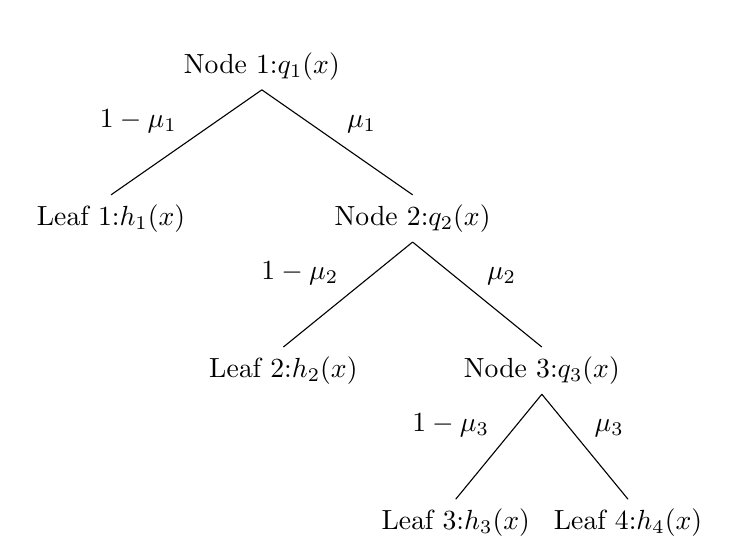
\begin{tikzpicture}[level distance=55pt]
\Tree
[.{Node 1:$q_1(x)$} 
	\edge node[auto=right] {$1 - \mu_1$};		
	[.{Leaf 1:$h_1(x)$} ] 
	\edge node[auto=left] {$\mu_1$};		
	[.{Node 2:$q_2(x)$} 
		\edge node[auto=right] {$1 - \mu_2$};	
		{Leaf 2:$h_2(x)$} 
		\edge node[auto=left] {$\mu_2$};	
		[.{Node 3:$q_3(x)$} 
			\edge node[auto=right] {$1 - \mu_3$};	
			{Leaf 3:$h_3(x)$} 
			\edge node[auto=left] {$\mu_3$};	
			{Leaf 4:$h_4(x)$} 
		] 
	] 
]
\end{tikzpicture}
}
\caption{Topology of Deepcascade SVM}
\label{topology}
\end{figure}
\\That is at each internal node, an SVM is trained on the incoming points. Then the closest fraction $\mu_k$ of points to the separating hyperplane are removed from the current set of points and sent to the next level for it to be trained with a new SVM with a possibly different kernel. The remainder of $1-\mu_k$ fraction of points stay classified by the same hyperplane which is treated as that particular leaf hypothesis.
%May not be needed
\\The pseudocode for the DeepCascadeSVM is as follows:
{\small \begingroup
\captionof{algorithm}{Deep Cascade SVM}
\endgroup
\begin{algorithmic}[1]
\Function {DeepCascadeSVM}{L,$\mathcal{M}$,$\gamma$}	
	\For{$l \in [1 \cdots L],(\mu_k)_{1 \leq k \leq l} \subseteq \mathcal{M},(\delta_k)_{1 \leq k \leq l} \subseteq \mathcal{G}$}
		\State{$S_1 \gets S$}
		\For{$ k = 1$ to $l$}
			\State{$h_k \gets$ SVM$(\delta_k,S_k)$}
			\State{$q_k \gets \arg_{q \in Q_k} \{ | q^{-1}(1) \cap S_k | = \mu_k |S_k| \}$}
			\State{$S_{k+1} \gets q_{k}^{-1}(1) \cap S_k$}
		\EndFor
		\State{$f(\cdot) \gets \sum_{k=1}^{l-1} \left( \prod_{j=1}^{k-1} q_j \right) \bar{q_k}h_k + \left( \prod_{j=1}^{l} q_j \right) h_l$}
		\State{$\mathcal{F} \gets \mathcal{F} \cup \{ f \} $}
	\EndFor
	\State{$f^* \gets \argmin_{f \in \mathcal{F}} \widehat{R}_s(f) + \sum_{k=1}^{l} \min \left( 4\gamma \left[ \sum_{j=1}^{d_k} \sqrt{\frac{d_{f,j} \log\frac{em}{d_{f,j}}}{m}} + \sqrt{\frac{d_{f,k} \log\frac{em}{d_{f,k}}}{m}} \right] , \frac{m_k^+}{m} \right) $}
\EndFunction
\end{algorithmic}
}
The deep cascade functions generated by the algorithm are based on repeatedly
 using SVMs combined with polynomial kernels of different degree. The
leaf hypothesis sets $H_k$ are decision surfaces defined by polynomial kernels (hyperplanes in the kernel hilbert space).
The hypothesis $h_k \in H_k$ is learned via the SVM algorithm with a polynomial
kernel of degree $\delta_k$ on subsample $S_k$ . The node question hypothesis set $Q_k$ is
the set of indicator functions which indicate if a point is within a distance $c$ from the hyperplane such that $\mu_k|S_k|$ points lie within that distance $c$ from the hyperplane. 
\\A search is done over all depths $[1 \cdots L]$, fraction of points $\mu_k \in \mathcal{M}$ and degree of kernels $\delta_k \in \mathcal{G}$ such that the resulting cascade minimizes the generalization error. We also see that the rademacher complexities from (\ref{dcbound}) have been bounded by the VC dimension of the respective SVM ($d_{f,j},d_{f,k}$) and that a factor $\gamma$ has been introduced to scale the hinge loss. Thus the DeepCascadeSVM only tries to get the minimal upper bound  in terms of the VC dimension rather than trying to minimize the rademacher complexities.


\subsection{Perceptron Algorithm}
The perceptron algorithm is one of a broad family of online learning algorithms and has quite a few variants. We are looking at the kernelized perceptron variant of the same. The original perceptron algorithm is an ``error driven'' algorithm that trains on the dataset to learn a separating linear homogeneous threshold function given as $w.x=0$. Each time a mistake is made on point $x_i$, $w$ is adjusted by $x_iy_i$. 
\\In the case of the kernelized perceptron we actually need to learn a hyperplane in the kernel hilbert space, for which we first need to identify the dual formulation. This is done by observing that $w$ can be expressed as  linear combination of the training samples. The equation being $w = \sum_{i=1}^{m} \alpha_i y_i x_i$. Then we can see that adjusting $w$ with $y_ix_i$ in the primal form is the same as adjusting the $\alpha_i$ by 1. Now we see that the predicted $\widehat{y}_i$ is given using $sgn(w\cdot x_i)$. Writing this with the dual we see that:
\par
{\footnotesize
\begin{equation}
\begin{aligned}
\widehat{y}_t &= sgn(w^T x_t)\\
&= sgn \left( \sum_{i=1}^{m} \alpha_i y_i x_i \right) ^T x_t\\
&= sgn \sum_{i=1}^{m} \alpha_i y_i (x_i \cdot x_t)
\end{aligned}
\end{equation}
}\par
Since it has come to a dot product form we can now use kernels to evaluate the same. This is the principle behind kernelized perceptron. Also this can be adapted to a batch setting by simply running the algorithm over all the points and repeating for a few passes if needed. The psuedocode is as follows:
{\small \begingroup
\captionof{algorithm}{Batch Kernelized Perceptron}
\endgroup
\begin{algorithmic}[1]
\Function {KernelizedPerceptron}{$S,K$}	\Comment{Where $S$ is the sample set and $K$ is the kernel}
	\State{$\alpha \gets \alpha^0$} \Comment{Where $\alpha^0$ is the $\alpha$ corresponding to the initial $w$,typically 0}
	\For{$p=1$ to $passes$}	
		\For{$t=1$ to $T$}
			\State{Receive($x_t \in S$)}
			\State{$\widehat{y}_t \gets sgn \sum_{i=1}^{m} \alpha_i y_i K(x_i,x_t)$}
			\State{Receive($y_t \in S$)}
			\If{$\widehat{y}_t \neq y_t$}
				\State{$\alpha_t \gets \alpha_t + 1$}
			\EndIf
		\EndFor
	\EndFor
	\State{\Return $\alpha$}
\EndFunction
\end{algorithmic}
}
The point to be noted with regards to perceptrons is the fact that training time for this is linear in the number of samples.

\section{Algorithm}
We have adapted the deep cascades to work with kernelized perceptrons serving as the leaf hypothesis and node questions. The adaptation is similar to the DeepCascadeSVM with a few subtle differences. The psuedocode is as follows:
{\small \begingroup
\captionof{algorithm}{Deep Cascade Kernelized Perceptron}
\endgroup
\begin{algorithmic}[1]
\Function {DeepCascadePerceptron}{$S,L,\mathcal{M},\mathcal{G},\gamma$}	
	\For{$l \in [1 \cdots L],(\mu_k)_{1 \leq k \leq l} \subseteq \mathcal{M},(\delta_k)_{1 \leq k \leq l} \subseteq \mathcal{G}$}
		\State{$S_1 \gets S$}
		\For{$ k = 1$ to $l$}
			\State{$h_k \gets$ KernelizedPerceptron$(S_k,poly\_kernel(\delta_k))$}
			\State{$threshold \gets c_k : |\{ x_t : \sum_{i=1}^{|S_k|} \alpha_i y_i K(x_i,x_t) \leq c_k \}| = \mu_k|S_k| $}	%\Comment{Gets the distance of $\mu_k$ fraction of closest point from hyperplane}
			\State{$q_k \gets 1_{\sum_{i=1}^{|S_k|} \alpha_i y_i K(x_i,x) \leq threshold}$}
			\State{$S_{k+1} \gets q_{k}^{-1}(1) \cap S_k$}
		\EndFor
		\State{$f(\cdot) \gets \sum_{k=1}^{l-1} \left( \prod_{j=1}^{k-1} q_j \right) \bar{q_k}h_k + \left( \prod_{j=1}^{l} q_j \right) h_l$}
		\State{$\mathcal{F} \gets \mathcal{F} \cup \{ f \} $}
	\EndFor
	\State{$f^* \gets \argmin_{f \in \mathcal{F}} \widehat{R}_s(f) + \sum_{k=1}^{l} \min \left( 4\gamma \left[ \sum_{j=1}^{d_k} \sqrt{\frac{d_{f,j} \log\frac{em}{d_{f,j}}}{m}} + \sqrt{\frac{d_{f,k} \log\frac{em}{d_{f,k}}}{m}} \right] , \frac{m_k^+}{m} \right) $}
\EndFunction
\end{algorithmic}
}
The sample set is standardized using standard scaling before being sent to the algorithm. This is done to center the data and normalize it. The same scaling is applied to the test data as well. This centered scaling becomes quite important in the case of perceptrons as it learns only a linear homogeneous threshold function.
\\The algorithm essentially consists of training perceptrons $h_k$ at each level (total of $l$ levels) with the incoming points using polynomial kernels of dimension $\delta_k$. Once the perceptron at level $k$ is trained on $S_k$, the distances to all points are measured as $w_k.x = \sum_{i=1}^{|S_k|} \alpha_i y_i K(x_i,x)$ (ignoring the factor of $\lVert w_k \rVert$ as we just want to get the $\mu_k$ fraction of closest points). With the distances calculated we decide on a threshold as the distance from the hyperplane such that $\mu_k|S_k|$ points lie within that distance. The node question is then: whether or not a given point lies within this threshold from the trained hyperplane. This process is then repeated for each level.
\\The algorithm generates multiple cascades for each of the depth $l \in [1 \cdots L]$, any sequence of fraction values $(\mu_k)_{1 \leq k \leq l} \subseteq \mathcal{M}$ and sequence of polynomial kernel degrees $(\delta_k)_{1 \leq k \leq l} \subseteq \mathcal{G}$. The node question and leaf hypothesis for these cascades are chosen as described above. Then the best cascade $f^*$ is chosen as the one that minimizes an upper bound on the generalization error bound of (\ref{dcbound}) similar to what is done for the DeepCascadeSVM \cite{deepcascades}. That is $f^*$ is chosen to minimize the bound:
\begin{equation}
R(f) \leq \widehat{R}_s(f) + \sum_{k=1}^{l} \min \left( 4\gamma \left[ \sum_{j=1}^{d_k} \sqrt{\frac{d_{f,j} \log\frac{em}{d_{f,j}}}{m}} + \sqrt{\frac{d_{f,k} \log\frac{em}{d_{f,k}}}{m}} \right] , \frac{m_k^+}{m} \right)
\label{dcvcbound}
\end{equation}
where $d_k$ is the depth of node $k$ and $d_{f,k}$ is the VC dimension of the perceptron trained at level $k$ and the $\gamma$ parameter is introduced to scale the loss function. %TODO:Re-check.
\\The VC dimension of a perceptron accepting samples of dimension $n$ and working with a polynomial kernel of degree $\delta$ is $\binom{n+\delta}{\delta}$. This can be seen by the definition of polynomial kernel: ($K(x,y) = (1+x \cdot y)^\delta$) and using multinomial theorem.
\\The $\gamma$ is selected by doing a n-fold cross validation to select the best $\gamma$ from a set of values.

\section{Experiments}
We performed some preliminary experiments on the \emph{breastcancer, ionosphere} datasets from UCI machine learning repository \cite{Lichman:2013}.
\\In our experiments we used the following parameters: max cascade depth $L=4$, the set of fraction values was chosen as $\mathcal{M} = \{ 0.2,0.4,0.6,0.8 \}$ and the degree of the kernels were chosen from $\mathcal{G} = \{ 1 \cdots 4 \}$.
\\We have split our dataset into a $80\%$ training set and $20\%$ test set. The training set was inturn split into 3 folds and for each fold leaving that out for validation we trained on the other two. This way a 3-fold cross validation was performed to figure out the correct $\gamma \in \{ 10^{-i} : i \in \{ 0,1,2,3 \} \}$.
\begin{table}[h]
\begin{tabular}{| l | l | l | l | l |}
\hline
Dataset & Number of examples & Number of features & DeepCascadePerceptron\\
&&&Validation error $\pm$ Deviation & SVM Validation error $\pm$ Deviation \\
\hline
breastcancer & 699 & 9 & 0.036 $\pm$ 0.008 & 0.027 $\pm$ 0.004 \\
ionosphere & 351 & 34 & 0.071 $\pm$ 0.032 & 0.093 $\pm$ 0.033 \\
\hline
\end{tabular}
\caption{Cross Validation error for DeepCascadePerceptron}
\end{table}

\begin{table}[h]
\begin{tabular}{| l | l | l | l | l |}
\hline
Dataset & Cascade Depth & DeepCascadePerceptron & SVM & Perceptron\\
\hline
breastcancer & 4 & 0.02 & 0.057 & 0.036 \\
ionosphere & 2 & 0.126 & 0.126 & 0.112 \\
\hline
\end{tabular}
\caption{Test error for DeepCascadePerceptron, SVM, Kernelized Perceptron run on the same set}
\end{table}


\section{Conclusions}
\nocite{fml}
\printbibliography
%%% End document
\end{document} 
